%%%%%%%%%%%%%%%%%%%%%%%%%%%%%%%%%%%%%%%%%%%%%%%%%%%%%%%%%%%%%%%%%%%%%%%%%%%%%%%
%%                                                    DATA SIMULATION SELECTION
%%%%%%%%%%%%%%%%%%%%%%%%%%%%%%%%%%%%%%%%%%%%%%%%%%%%%%%%%%%%%%%%%%%%%%%%%%%%%%%
%%                                    about the samples, MC Generation and cuts 



%______________________________________________________________________________
%                                                Daten Simulation und Selektion 
\chapter{Daten, Simulation \texorpdfstring{\&}{und} Selektion}

\begin{quote}
    Die Grundlage jeder wissenschaftlichen Arbeit ist die Datenerhebung. In
    diesem Kapitel wird zunächst kurz auf die Parameter des Beschleunigers und
    des Detektors während der Aufzeichnung der Daten eingegangen und der
    erhobene Datensatz charakterisiert. Anschließend werden Aspekte der
    vergleichenden Monte-Carlo Simulation erörtert und die in dieser Arbeit
    benutzten simulierten Datensätze vorgestellt. Abschließend werden noch eine
    Reihe von Selektionskriterien erläutert, die aus der Gesamtheit der
    erhobenen Daten die für die folgende Analyse interessanten Informationen
    filtern.
\end{quote}



%______________________________________________________________________________
%                                                                         Daten 
\section{Daten}
\label{data_sim_selection:data}

% + Daten von 2012
% + Parameter: Energie, Bunchespacing, Perioden
% + Energie-Kalibration

Die Daten, die dieser Arbeit zugrunde liegen, wurden vom ATLAS-Detektor im Jahr
2012 bei erstmalig $8 \TeV$ Schwerpunktsenergie aufgenommen. Der \ac{LHC} wird
mit Paketen von Protonen, sogenannte Bunches (vom engl. Bunch: Bündel) gefüllt,
die für einige Stunden im Beschleuniger zirkulieren\footnote{weitere Details:
siehe Kapitel \ref{lhc}}. Eine solche Füllung steht für größtenteils identische
Einstellungen des Beschleunigers bzw. Detektors und wird in ATLAS mit einer
fortlaufenden Nummer identifiziert. Die Füllungs-Nummern größerer Perioden
konstanter Bedingungen, wie die zu der Zeit implementierten Trigger oder
globale \ac{LHC} Parameter, werden dann mit einem Buchstaben zusammengefasst
(Periode A, B, ...).

Der vorliegende Datensatz wurde in der Zeit zwischen dem 04. April 2012 und dem
16. Dezember 2012 aufgenommen und umfasst 10 Perioden, die einer integrierten
Gesamtluminosität von $20,3 \fb^{-1}$ entsprechen\footnote{nach Anwendung der
\ac{GRL} (siehe Kapitel \ref{data_sim_selection:selection})} (siehe Abbildung
\ref{fig:lumi}). Der Beschleuniger wurde hierbei in einer Konfiguration
betrieben, die einen zeitlichen Abstand zwischen den Teilchen-Paketen von
$50\:\nano\second$ gewährleistet, woraus eine instantane Luminosität von bis zu
$7,73 \cdot 10^{-33} \centi\meter^{-2}\second^{-1}$ resultiert.

Eine hohe instantane Luminosität verspricht eine große Rate interessanter
Ereignisse, jedoch bedingt sie auch viele unerwünschte Neben-Ereignisse, aus
inelastischen Streuprozessen, die einen signifikanten Einfluss auf die Messung
nehmen können. Dieser Effekt wird als \textit{Pile-Up} bezeichnet und ist in
Abbildung \ref{fig:pileup} illustriert.

\begin{figure}
    \begin{minipage}[b]{0.48\textwidth}
        \centering
        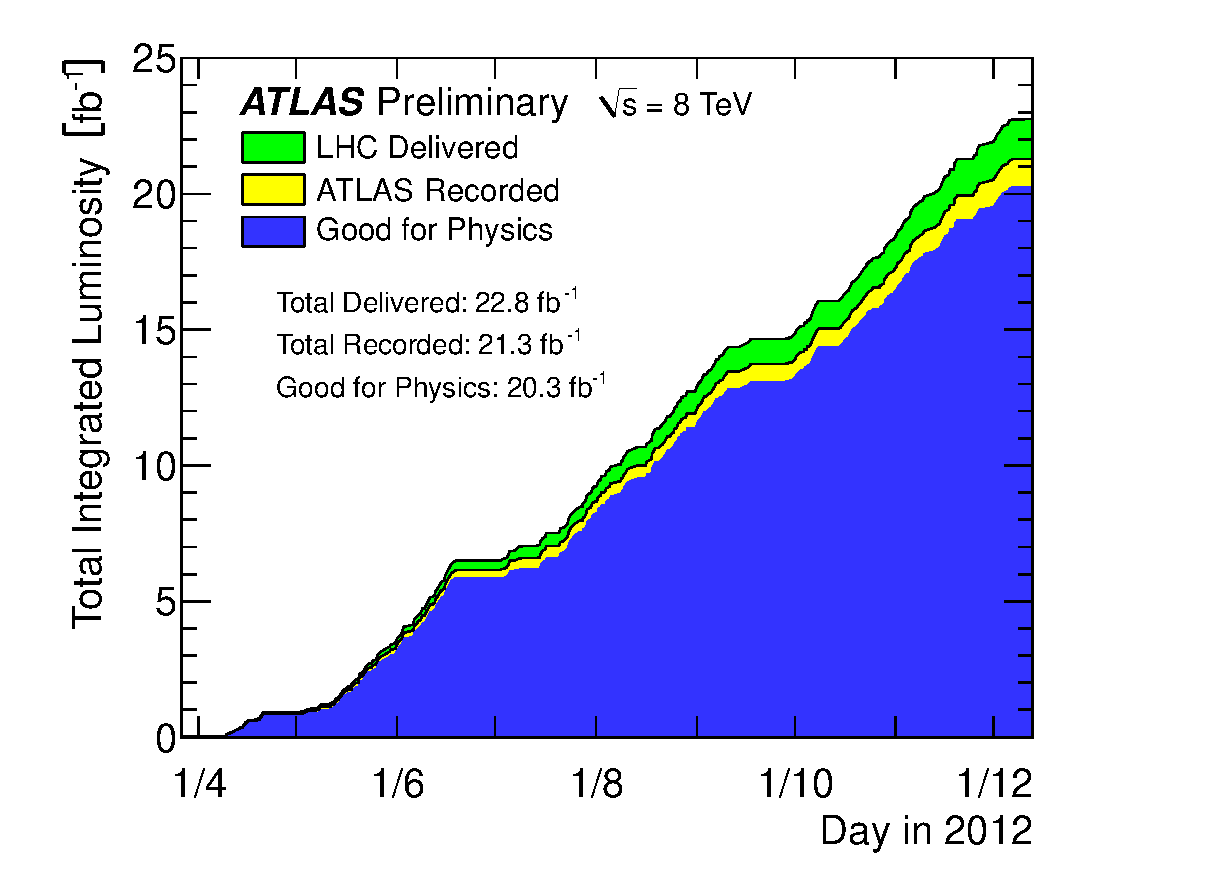
\includegraphics[width=1.\textwidth]{plots/lumi}
        \captionsetup{format=plain}
        \caption[Verfügbare, aufgezeichnete und validierte integrierte
            Luminosität aufgetragen gegen die Zeit]
            {Verfügbare, aufgezeichnete und validierte integrierte
            Luminosität aufgetragen gegen die Zeit innerhalb der Messkampagne.
            Quelle: \cite{ATLAS:Public}}
        \label{fig:lumi}
    \end{minipage}
    \hfill
    \begin{minipage}[b]{0.48\textwidth}
        \centering
        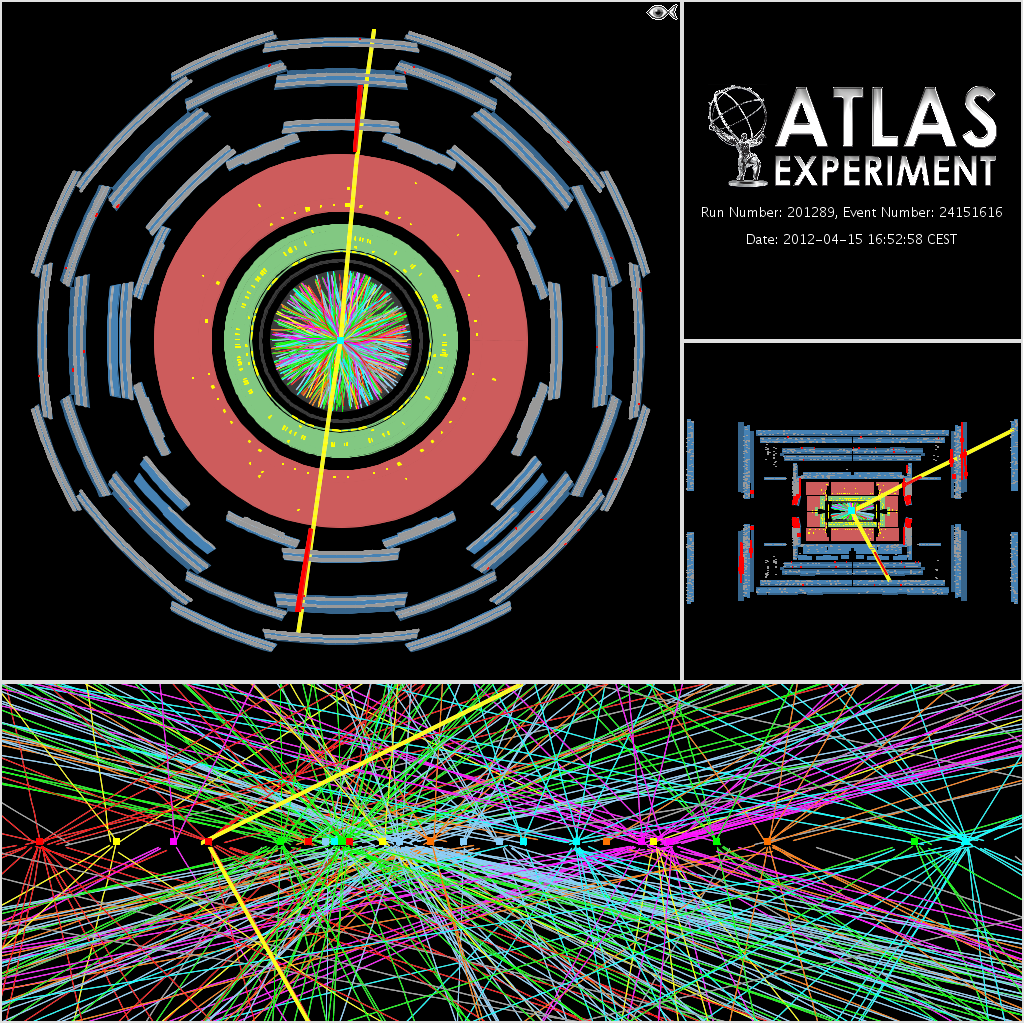
\includegraphics[width=1.\textwidth]{img/pileup}
        \captionsetup{format=plain}
        \caption[Ereignisse mit $Z \rightarrow \mu\mu$ Kandidat und hohem
            Pile-Up]
            {Ereignisse mit $Z \rightarrow \mu\mu$ Kandidat und hohem Pile-Up
            (25 rekonstruierte Vertizes). Quelle: \cite{ATLAS:Public}}
        \label{fig:pileup}
    \end{minipage}
\end{figure}

Das in dieser Arbeit verwendete Speicherformat für Daten basiert auf dem in
Abschnitt \ref{trigger_daq} beschriebenen DPD Format. Für die Verwendung
innerhalb der Arbeitsgruppe in Mainz wurden diese Tupel zum Zwecke der
Speicherplatz-Ersparnis auf Ereignisse beschnitten, die mindestens zwei
Elektronkandidaten mit je $23 \GeV$ bzw. $14 \GeV$ aufweisen.

Die Energie der Elektronkandidaten in diesen Tupeln beruht auf der Information
aus den Rekonstruktionsalgorithmen und bedarf noch der Kalibration. Für
Elektronen im Zentral-Bereich werden dazu Kalibrations-Faktoren benutzt, die
von der zuständigen ATLAS Arbeitsgruppe für die Kalibration des
elektromagnetischen Kalorimeters (\textit{Electron Gamma Working Group}, kurz:
egamma) bereitgestellt werden. Für Elektronen im Vorwärts-Bereich wurden noch
keine Kalibrations-Faktoren bereitgestellt, weshalb diese in Kapitel
\ref{energy_calibration} dieser Arbeit selbst bestimmt werden.



%______________________________________________________________________________
%                                                                    Simulation
\section{Simulation}
\label{data_sim_selection:simulation}

% + Motivation für Simulation (Theorie-Vorhersage)
% + Mehrschrittiges Prinzip
% + Eventgeneration (Matrixelemente, Fragmentation,...)
% + Detektorsimulation (+ Ausgabeformat)
% + Nötige Korrekturen (Pileup, Effizienzen, Smearing, kFaktors)
% + Übersicht und kurze(!) Statements zu Samples
% + LumiScaling

Die Simulation von Ereignissen und des Detektors ist ein wichtiger Bestandteil
von Analysen in der Hochenergiephysik. Sie repräsentiert einerseits das
beste Wissen über die betrachteten Prozesse und die genaue Kenntnis des
Detektors, andererseits lassen sich mit Simulationen die Erweiterungen durch
neue theoretische Modelle untersuchen und deren Einfluss auf bereits bekannte
Prozesse vorhersagen. Zentraler Gegenstand der Betrachtung ist hierbei stets
der Vergleich zwischen Simulation und realen Daten.



\subsection{Erzeugung simulierter Datensätze}
\label{event_generation}
Die Erstellung einer Simulation, im folgenden meist nur noch als
\textit{Monte-Carlo} bezeichnet, geschieht für gewöhnlich in mehreren
Schritten. Eine grobe Unterteilung ist die Unterscheidung zwischen der
Simulation des eigentlichen physikalischen Prozesses, wie beispielsweise die
Annihilation eines Quarks und eines Antiquarks in Proton-Proton Kollisionen zu
einem Z-Boson und dessen nachfolgenden Zerfall in ein Leptonpaar, und die
Simulation der Detektorantwort, also der Beschreibung aller physikalischer
Subprozesse, die von den Produkt-Teilchen im Detektor induziert werden
(Detektor-Antwort).

Im ersten Schritt, der Ereignis-Simulation, kommen so genannte
\textit{Monte-Carlo Generatoren} zum Einsatz. Dies sind konfigurierbare
Software Pakete, die mittels Zufallsmethoden die gewünschten Prozesse, samt der
kinematischen Parameter der eingehenden und ausgehenden Teilchen als Ereignisse
simulieren. Dies geschieht auf der Basis von theoretischen
Wirkungsquerschnitten und der Definition des Phasenraumes. Die voran gestellte
Berechnung der Matrixelemente\footnote{siehe auch Kapitel
\ref{theory:electroweak}} findet meist in führender (LO) oder nächst-führender
(NLO) Ordnung statt. Betrachtungen höherer Ordnungen werden aufgrund der
übermäßigen Komplexität in der Regel durch Umgewichtungen von Simulationen
niedrigerer Ordnung durch sogenannte \textit{kFaktoren}
realisiert\footnote{siehe auch Abschnitt \ref{mc_corrections}}, zu deren
Bestimmung das Verhältnis der Wirkungsquerschnitte der höheren und niedrigeren
Ordnung gebildet wird. Neben dem harten Streuprozess inklusive aller
beteiligten Partonen und möglichen Zerfallsprodukten werden anschließend
weitere Effekte wie beispielsweise Hadronisierung oder Bremsstrahlung
berücksichtigt. Alle bis zu diesem Punkt gewonnenen Werte bezeichnet man als
\textit{Generator-Level}.

Die kinematische Information der Teilchen im Endzustand auf Generator-Level
wird nun der Detektor-Simulation übergeben, welche die Wechselwirkung mit
Detektormaterial und die elektronische Antwort des Detektors beschreibt, sodass
an deren Ende ein mit realen Signalen vergleichbarer Datensatz entsteht. Diese
Aufgabe übernimmt in ATLAS das \textsc{GEANT4}-Paket
(\cite{Agostinelli:2002hh}), mithilfe dessen eine sehr detailgetreue virtuelle
Beschreibung des Detektors erstellt wurde.



\subsection{Korrekturen}
\label{mc_corrections}
Die reine Simulation des Streuprozesses und der Antwort des Detektors ist zwar
eine gute Annäherung an die realen Verhältnisse, allerdings treten bei genauer
Betrachtung Diskrepanzen auf, die es zu korrigieren gilt. Die Ursache für die
Unterschiede liegt meist in der Abhängigkeit schwierig simulierbarer Größen,
wie zum Beispiel das oben beschriebene Pile-up aber auch Beiträge durch 
Prozesse hoher Ordnung. Um dennoch sinnvolle Vergleiche zwischen Daten und
Monte-Carlo anstellen zu können werden die simulierten Datensätze umgewichtet.
So gibt es für jede Korrektur einen Satz sogenannter Skalenfaktoren, die jedem
simulierten Ereignis ein oftmals von 1 verschiedenes Gewicht zuordnen.

Im Folgenden wird eine kurze Übersicht über die möglichen Korrekturen gegeben:

\begin{description}
    \item[Pile-Up:] Der oben beschriebene Effekt des Pile-Up, also der
        gleichzeitig stattfindenden zusätzlichen Teilchen-Kollisionen ist nur
        schwer vorhersagbar. Deshalb wird die Pile-Up Verteilung der
        Monte-Carlo Simulationen auf die entsprechende Verteilung der
        gemessenen Daten umgewichtet. Die dafür nötigen Ereignis-Gewichte
        werden im Folgenden mit $w_\text{pu}$ bezeichnet.
    \item[Energieauflösung:] Die Simulation der Detektor-Antwort nimmt die
        Energieauflösung des Kalorimeters\footnote{Aufgrund der Thematik dieser
        Arbeit ist nur die Auflösung des elektromagnetischen Kalorimeters
        relevant und hier gemeint} oftmals zu optimistisch an, sodass eine
        zusätzliche Energieverschmierung eingeführt wird, um dies zu
        korrigieren. Die Bestimmung der Korrektur-Faktoren ist Teil dieser
        Arbeit und wird in Kapitel \ref{energy_calibration} besprochen.
    \item[Elektron-Rekonstruktions-Effizienz:] Die Effizienz mit der Elektronen
        im ATLAS-Detektor rekonstruiert werden ist nicht einfach zu
        beschreiben, weshalb hier zusätzlich Skalenfaktoren pro betrachtetem
        Elektron notwendig werden. Man führt insgesamt drei Korrekturfaktoren
        ein um die Effizienz des \textit{Triggers} ($w_\text{trigger}$), der 
        \textit{Spur-Rekonstruktion} ($w_\text{spur}$) und der
        \textit{Identifikation} ($w_\text{ID}$) zu korrigieren, wobei die
        beiden erstgenannten aufgrund der Abwesenheit von Trigger und
        Spurinformation im Vorwärts-Bereich\footnote{siehe hierzu auch Kapitel
        \ref{atlas_detector}} nicht für Vorwärts-Elektronen definiert sind.
    \item[kFaktoren:] Als kFaktoren bezeichnet man die Skalenfaktoren, die der
        Umgewichtung eines simulierten Datensatzes auf die nächst höhere
        Ordnung dienen also beispielsweise NLO $\rightarrow$ NNLO. Sie werden
        pro Ereignis angewendet und hängen meist von der jeweiligen
        invarianten Masse ab. Im Folgenden werden sie mit $w_\text{kFactor}$
        bezeichnet.
    \item[Vertex-Position:] Die Position des Wechselwirkungspunktes hat
        Einfluss auf die Rekonstruktion der Elektronen und zählt ebenfalls zu
        den schwer zu simulierenden Größen. Skalenfaktoren ($w_\text{vtx}$)
        korrigieren ereignisweise die Verteilung im Monte-Carlo.
    \item[Generator-Ereignisgewicht:] Einige Monte-Carlo Generatoren,
        insbesondere jene, die Ereignisse auf nächst-führender Ordnung
        simulieren, setzen für manche der erzeugten Ereignisse ein Gewicht
        abweichend von 1 fest, um intrinsische Doppelzählung zu korrigieren.
        Diese Gewichte ($w_\text{gen}$) werden mit den sonstigen Gewichten
        multipliziert.
\end{description}

Für alle hier beschriebenen Korrekturen, mit Ausnahme der
Generator-Ereignis"-gewichte, werden von den zuständigen Arbeitsgruppen in ATLAS
Software-Pakete bereitgestellt, die alle benötigten Skalenfaktoren beinhalten
und regelmäßig auf den Stand neuester Erkenntnis aktualisiert werden.



\subsection{Benutzte Monte-Carlo Simulationen}
\label{used_mc_samples}
Die meisten in dieser Arbeit verwendeten Monte-Carlo Simulationen werden von
der ATLAS \textit{Monte-Carlo Working Group} produziert und
verifiziert\footnote{alle eigens generierten Monte-Carlo Simulationen werden
gesondert gekennzeichnet}. Sie unterscheiden sich vor allem in der Wahl des
Generators und des simulierten Prozesses, durchlaufen aber ausnahmslos dieselbe
Detektorsimulation.

Eine Übersicht über die verschiedenen Prozesse und Generatoren wird im
folgenden gegeben und ist in Anhang \ref{appendix:monte_carlo_samples}
zusammengefasst; detailliertere Informationen über die Motivation und die
tatsächliche Verwendung der jeweiligen Monte-Carlos wird später in den
betreffenden Kapiteln gegeben.

\subsubsection*{Drell-Yan}
Die wichtigste Monte-Carlo Simulation ist die des in dieser Arbeit betrachteten
Signalprozesses $q\bar q \rightarrow \gamma^*/Z \rightarrow e^+e^-$ zu deren
Produktion eine Kombination der beiden Generatoren \textsc{Powheg}
(\cite{Alioli:2010xd}) und \textsc{Pythia8} (\cite{Sjostrand:2007gs}) benutzt
wurde. \textsc{Powheg} übernimmt dabei die Simulation des eigentlichen
Streu-Prozesses auf nächst-führender Ordnung (NLO) und übergibt die
Partoninformation an \textsc{Pythia8}, welches dann die weiteren Prozesse, wie
Hadronisierung simuliert. Es wurden neben einem inklusiv in der invarianten
Masse generierten Monte-Carlo mit etwa 10 Millionen Ereignissen auch auf höhere
Massenbereiche eingeschränkte Monte-Carlos mit jeweils 1 Million Ereignissen
produziert, um auch in hohen invarianten Massenbereichen ausreichend
statistische Signifikanz zu gewährleisten. Das erste dieser massenbeschränkten
Monte-Carlos hat eine untere Grenze von $m_{ee} > 120 \GeV$, sodass bei
gleichzeitiger Verwendung mit dem inklusiv generierten Monte-Carlo letzteres an
dieser Grenze auf Generator-Level abgeschnitten werden muss. Die Arbeitsgruppe
für die Suche nach schweren Eichbosonen in ATLAS (\textit{ZPrime}) stellt für
diese Monte-Carlos massenabhängige kFaktoren bereit, die die bestehende
Simulation auf NNLO umgewichten.

Ebenso sind für den verwandten Prozess
$q\bar q \rightarrow \gamma^*/Z \rightarrow \tau^+\tau^-$ analog zu obiger 
Herangehensweise und Konfiguration Monte-Carlos produziert worden, die in
der vorliegenden Arbeit zur Abschätzung des Untergrundes durch diesen Prozess
verwendet werden\footnote{$\tau$-Leptonen zerfallen mit gewisser
Wahrscheinlichkeit in Elektronen}. Die Schnittgrenze zwischen den
massenbeschränkten und dem inklusiv produzierten Monte-Carlo liegt hier
allerdings etwa doppelt so hoch, bei $250 \GeV$.

\subsubsection*{W+Lepton}
Der Zerfall eines W-Bosons in ein Elektron bzw. Positron und ein entsprechendes
(Anti-)Neutrino oder in ein $\tau^+/\tau^-$ und ein entsprechendes
(Anti-)Neutrino wird mit der selben Kombination von Generatoren, wie schon beim
Drell-Yan Prozess simuliert und dient ebenfalls der späteren
Untergrundabschätzung. Jeder der eben genannten Prozesse wurde zu diesem Zweck
separat simuliert. Für den Zerfall in Elektronen/Positronen wurden dabei
jeweils etwa 40 Millionen und für den Zerfall in $\tau^+/\tau^-$ je 7
Millionen Ereignisse generiert.

\subsubsection*{Top-Produktion}
Die Produktion eines einzelnen Top-Quarks oder eines Paares von Top-Quarks und
deren Zerfall sind relevante Prozesse für die Abschätzung des Untergrundes der
späteren Analyse. Top-Quarks zerfallen mit fast 100\% Verzweigungsverhältnis in
ein b-Quark und ein W-Boson, wobei letzteres wie oben beschrieben in ein Lepton
und ein entsprechendes (Anti-)Neutrino zerfallen kann.

Abbildung \ref{fig:singletop} zeigt die möglichen Produktionskanäle für ein
einzelnes Top-Quark. Für jeden der gezeigten Kanäle (a,b,c) wurde ein separates
Monte-Carlo generiert, wobei für (a) und (b) jeweils noch zwischen dem
konsekutiven Zerfall des $W$-Boson in ein Elektron/Positron und ein
$\tau^+/\tau^-$ unterschieden wurde.

\begin{figure}
    \centering
    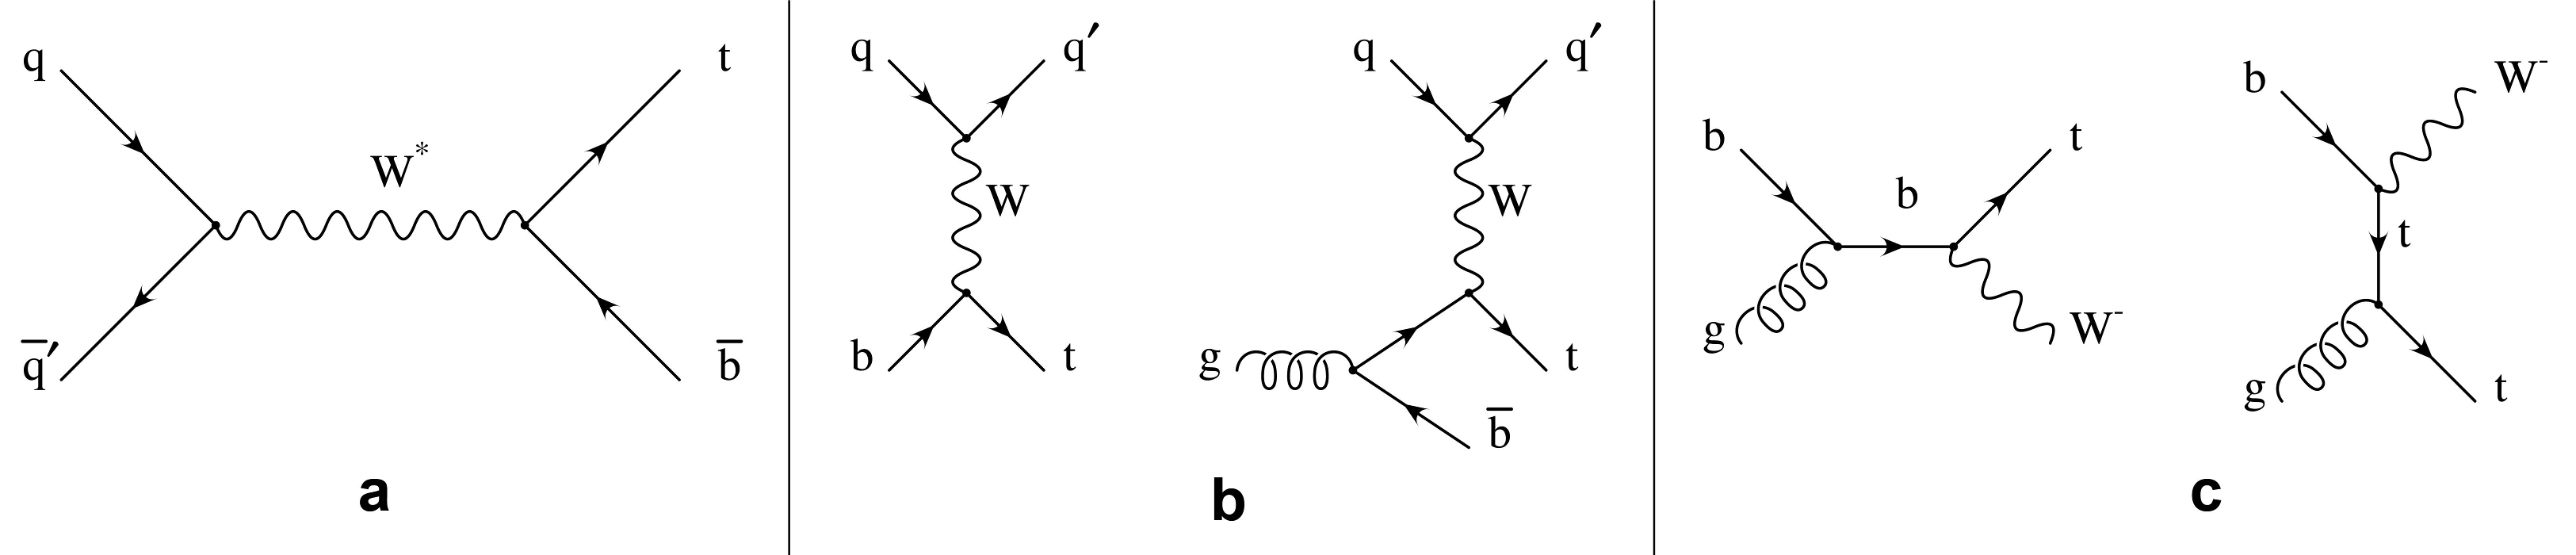
\includegraphics[width=1.\textwidth]{img/singletop}
    \caption[Produktionskanäle für ein einzelnes Top-Quark in Proton-Proton
        Kollisionen]
        {Produktion eines einzelnen Top-Quarks in Proton-Proton Kollisionen im
        s-Kanal (a), t-Kanal(b) und mit einem W-Boson im Ausgangszustand (c).}
    \label{fig:singletop}
\end{figure}

Für die Produktion im t-Kanal (b) wurde für die Simulation des Streuprozesses
\textsc{AcerMC} (\cite{Kersevan:2004yg}) als Generator verwendet, der eine
Schnittstelle zu \textsc{Pythia6} (\cite{1126-6708-2006-05-026}) zur
Beschreibung der Hadronisierung bereitstellt. Die beiden anderen Kanäle (a) und
(c) und die Produktion eines Top-Antitop Paares wurden hingegen mit
\textsc{MC@NLO} (\cite{Frixione:2002ik}) simuliert, einem Generator, der in der
Lage ist, auf nächstführender Ordnung \ac{QCD} Prozesse zu simulieren. Für die
Top-Antitop Paarproduktion konnte von der oben bereits erwähnten
\textit{ZPrime} Gruppe der Wirkungsquerschnitt auf NNLO berechnet
werden\footnote{Die Wirkungsquerschnitte aller verwendeten Monte-Carlos ist in
Anhang \ref{appendix:monte_carlo_samples} zu finden}, was bei der weiter unten
beschriebenen Skalierung der Monte-Carlos relevant wird.

\subsubsection{Diboson}
Weitere Beiträge zur Untergrundabschätzung liefert die Simulation von der
Produktion zweier schwerer Eichbosonen. Dabei werden für jede Kombination, also
WW/WZ/ZZ separate Monte-Carlos generiert. Der hierfür verwendete Generator ist
\textsc{Herwig++} (\cite{Bahr:2008pv}), der in führender Ordnung die
Streuprozesse und die Hadronisierung simuliert. Auch für diese Simulationen
konnten von der \textit{ZPrime} Gruppe die Wirkungsquerschnitte auf NLO
berechnet werden.



\subsection{Skalierung}
Die generierten Monte-Carlo Simulationen entsprechen mit ihren
unterschiedlichen Wirkungsquerschnitten und der Zahl generierter Ereignisse
verschiedenen integrierten Luminositäten, weshalb zum Vergleich mit realen
Daten eine Skalierung notwendig wird. Man normiert dabei alle aus Monte-Carlos
erstellten Histogramme auf die äquivalente Luminosität in den Daten, mit einem
Skalierungsfaktor $s$:

\begin{equation}
    s = \frac{\sigma\cdot\epsilon\cdot L}{\sum_i^N w_{\text{pu},i}\cdot
    w_{\text{gen},i}}
    \label{eq:mc_scaling}
\end{equation}

Dabei bezeichnet $\sigma$ den Wirkungsquerschnitt des generierten Monte-Carlos
und $L$ die integrierte Luminosität des Datensatzes, auf den skaliert wird,
also im vorliegenden Fall $20.3 \fb^{-1}$. Anstelle durch die Gesamtzahl der
generierten Ereignisse zu dividieren, müssen die nicht-unitären Gewichte, wie
Pile-Up und Generator-Ereignisgewicht, berücksichtigt werden und durch deren
Produkt, summiert über alle Ereignisse, geteilt werden. Bei einigen der
erzeugten Monte-Carlos wurde ein zusätzlicher Filter eingesetzt, um nicht
relevante Ereignisse\footnote{zum Beispiel Ereignisse deren Produktteilchen
nicht im angestrebten Phasenraum zu finden sind} zu unterdrücken. Die Effizienz
dieser Filter wird mit $\epsilon$ berücksichtigt.

Alle Ereigniszahlen, Wirkungsquerschnitte und Effizienzen sind in Anhang
\ref{appendix:monte_carlo_samples} in den jeweiligen Tabellen zu den
Monte-Carlo Simulationen zu finden.



%______________________________________________________________________________
%                                                                     Selektion 
\section{Selektion}
\label{data_sim_selection:selection}

% + Motivation für Schnitte (Untergrund-Diskriminierung)
% + Event-basierte Schnitte (Trigger, Detektor, primVertex)
% + Elektron-basierte Schnitte (CC/CF, pT, ID, Autor, IQ)
% + kurze erwähnung andere schnitte (MET,Jets,...)

Als \textit{Selektion} bezeichnet man die Gesamtheit von Kriterien, deren
Anwendung auf die vollständige Ereignismenge eines Datensatzes zu jener
Teilmenge von Ereignissen führt, die nur noch für die angestrebte Analyse
relevante Informationen enthält. Dies dient der Unterdrückung von
Untergrundbeiträgen und der gleichzeitigen Anreicherung mit Signalereignissen.
Als Kriterien kommen vielfältige Bedingungen an die enthaltenen Teilchen oder
das Ereignis an sich in Frage. Die einfachste und zugleich meist genutzte Form
solcher Bedingungen sind simple Schnitte, bei denen einer Observablen ein
fester Grenzwert zugewiesen wird und ein Über- oder Unterschreiten dieses
Wertes das Verwerfen des Ereignisses bedingt. Auch komplexere Forderungen sind
denkbar, wie beispielsweise die logische Verkettung von Ja/Nein-Entscheidungen
(siehe z.B. Trigger-Entscheidungen, Abschnitt \ref{trigger_daq})
oder mehrdimensionale Schnittwerte auf der Basis multivariater Studien (siehe
Vorwärts-Elektron Identifikation, Abschnitt \ref{identification}).

Man kann grob zwei Klassen von Kriterien unterscheiden, jene die sich auf das
Ereignis als ganzes beziehen und solche, die auf Eigenschaften einzelner
Teilchen(-kanditaten) abzielen. Die folgende Übersicht zeigt die in dieser
Arbeit angewendeten Selektionkriterien und folgt dabei der derselben
Chronologie, wie sie auch in der späteren Analyse eingehalten wurde.

\begin{description}
    \cutitem{Good-Run-List (GRL)}{nur auf Daten}{Ereignis-Kriterium}
        Während der Datennahme muss sicher gestellt werden, dass alle
        Komponenten des Detektors innerhalb normaler Parameter arbeiten. Die
        Good-Run-List ist ein Verzeichnis mit dem dies dokumentiert wird. Hier
        sind alle Ereignisse\footnote{genauer die fortlaufende Nummer von
        Gruppen von Ereignissen} gelistet, die zur physikalischen Analyse
        verwendet werden können. Die hier benutzte \ac{GRL} trägt die ATLAS
        interne Bezeichnung
        \begin{verbatim}
    data12_8TeV.periodAllYear_DetStatus-v61-pro14-02_
    DQDefects-00-01-00_PHYS_StandardGRL_All_Good_
    EgammaForward.xml \end{verbatim}
        und steht für bestmögliche Detektor-Bedingungen inklusive der
        elektromagnetischen Kalorimeter im Vorwärts-Bereich.

    \cutitem{Trigger}{Daten \& Simulation}{Ereignis-Kriterium}
        Wie schon in Kapitel \ref{trigger_daq} erklärt, reduziert die Wahl des
        richtigen Triggers die Gesamtzahl der Ereignisse auf eine überschaubare
        Teilmenge, welche nur noch jene Ereignisse enthält, die bestimmten
        grundlegenden Anforderungen genügen und somit für die angestrebte
        Analyse als interessant gelten. Hierdurch findet bereits eine enorme
        Unterdrückung von Untergrund-Prozessen statt. Die von der
        \textit{egamma}-Gruppe empfohlene Trigger-Konfiguration für Analysen
        mit einem Elektronkandidaten ist die Verknüpfung durch ein logisches
        \emph{ODER} der beiden \acl{HLT}
        \begin{verbatim}
    e24vhi_medium1   (oder)   e60_medium1 \end{verbatim}
        Darin steht \texttt{eXX} für das Passieren der \acf{EF}
        Triggerentscheidung eines Elektronkandidaten mit Transversal-Impuls
        größer \texttt{XX} $\GeV$. Die Bezeichnung \texttt{medium1}
        repräsentiert das Äquivalent zur Identifikationsstufe\footnote{siehe
        Kapitel \ref{identification}} \textit{medium++} und der Anhang
        \texttt{vhi} fordert einen isolierten\footnote{d.h. ohne Überlapp des
        Elektron-Clusters mit einer benachbarten Energiedeposition im
        Kalorimeter} Elektronkandidaten, ohne Energiedeposition im dahinter
        liegendenden hadronischen Kalorimeter.

\pagebreak

    \cutitem{Spuren in Primärvertex}{Daten \& Simulation}{Ereignis-Kriterium}
        Als letztes ereignisbasiertes Kriterium wird die Anforderung an den
        Primärvertex gestellt Ausgangspunkt \textbf{mehr als 2 rekonstrukierter
        Spuren} zu sein. Dies dient der Verbesserung der Positionsbestimmung
        des Vertex und erhöht die Qualität der Zuordnung der Teilchenspuren.

    \cutitem{Pseudorapidität}{Daten \& Simulation}{Elektron-Schnitt}
        Die in Kapitel \ref{calorimeter} dargelegte Geometrie des Detektors
        initiierte die Unterscheidung zwischen Zentral- und
        Vorwärts-Elektronen. Eben diese Trennung macht eine Klassifizierung der
        Ereignisse in Zentral-Vorwärts, das heißt ein Elektron wird im
        Zentral-Bereich, das andere im Vorwärts-Bereich rekonstruiert und
        Zentral-Zentral, also beide Elektronen im Zentral-Bereich, sinnvoll.
        Der Einfachheit halber werden diese beiden Klassen im Folgenden
        entsprechend ihrer englischen Übersetzung mit \emph{CC}
        (central-central) und \emph{CF} (central-forward) abgekürzt. 

        Die Schnitte auf die Elektronkandidaten sind analog zur
        Detektor-Geometrie gewählt, wobei die Übergangsregionen zwischen den
        Kalorimetern exkludiert wurden.
        \begin{table}[h!]
            \centering
            \begin{tabular}{|c|c|c|}
                \hline
                \bf{Bereich} & \bf{Akzeptiert} & \bf{Exkludiert} \\
                \hline \hline
                Zentral  & $|\eta| < 2,47$      & $1,37 < |\eta| < 1,52$ \\
                Vorwärts & $2,5 < |\eta| < 4,9$ & $3,16 < |\eta| < 3,35$ \\
                \hline
            \end{tabular}
        \end{table}

        Durch diese Exklusion der Übergangsregionen wird gewährleistet, dass
        sich die Schauer der Elektronkandidaten innerhalb des aktiven
        Kalorimetermaterials entwickeln und so ein Energieverlust in den
        schlecht instrumentierten Bereichen unterbunden wird.


    \cutitem{Transversalimpuls}{Daten \& Simulation}{Elektron-Schnitt}
        Der Schnitt auf den Transversalimpuls der Elektronkandidaten reduziert
        vor allem die Untergrundbeiträge durch niederenergetische Jets. Während
        die kinematischen Kriterien des Triggers lediglich für
        Zentral-Elektronen greifen, verlangt dieser Schnitt die zusätzliche
        Konformität der Vorwärts-Elektronen. Bei der Wahl des Schnittwertes ist
        darauf zu achten, dass dieser oberhalb der intrinsischen
        Trigger-Schwelle liegt, um zu gewährleisten, dass die Selektion nicht
        jene Elektronkandidaten ausschließt, die zu einer positiven
        Trigger-Entscheidung geführt haben.

        In dieser Arbeit wurden zwei Konfigurationen von Grenzwerten für den
        Schnitt auf den Transversalimpuls verwendet; die Motivation für die
        spezielle Wahl der Schnittwerte wird in den entsprechenden Kapitel
        gegeben.

        Für die eigentliche Analyse, der Messung der Vorwärts-Rückwärts
        Asymmetrie (Kapitel \ref{afb})
        wurde ein Grenzwert von \emph{$30\GeV$} symmetrisch für Zentral- und
        Vorwärts-Elektronen gewählt.

        Die voran gestellte Energiekalibration der Elektronen in Kapitel
        \ref{energy_calibration} verwendet hingegen asymmetrische Bedingungen
        von \emph{$25\GeV$} für Zentral-Elektronen und \emph{$20\GeV$} für
        Vorwärts-Elektronen.

    \cutitem{Autor}{Daten \& Simulation}{Elektron-Schnitt}
        Mit diesem Kriterium wird sichergestellt, dass die Elektronkandidaten
        vom jeweils korrekten Rekonstruktionsalgorithmus\footnote{die
        Rekonstruktionsalgorithmen wurden in Kapitel \ref{reconstruction}
        erläutert} analysiert wurden. Diese tragen eine interne eindeutige
        Nummer, den sogenannten Autor, die während der Rekonstruktion in die
        Teilchenattribute eingetragen wird. Es werden deshalb für jeden
        Elektronkandidaten abhängig von seiner Klassifizierung (Zentral- oder
        Vorwärts-Elektron) folgende Bedingungen gestellt:
        \begin{table}[h!]
            \centering
            \begin{tabular}{|c|c|}
                \hline
                \bf{Bereich} & \bf{Autor} \\
                \hline \hline
                Zentral  & 1 \textit{oder} 3 \\
                Vorwärts & 8                 \\
                \hline
            \end{tabular}
        \end{table}

    \cutitem{Identifikation}{Daten \& Simulation}{Elektron-Schnitt}
        Dieser Schnitt legt die Identifikationsstufe für die Elektronkandidaten
        fest. Diese wurden in Kapitel \ref{identification} definiert und
        unterscheiden sich in 3 Kategorien. Für die vorliegende Arbeit wurde,
        wenn nicht explizit abweichend notiert, sowohl für Zentral- als auch
        für Vorwärts-Elektronen das höchste Niveau der Identifikation
        gefordert, also \textbf{\textit{tight++}} bzw.
        \textbf{\textit{fwdTight}}, was die größte Diskriminierung gegen
        andersartige Teilchen gewährleistet.

\pagebreak

    \cutitem{Ladung}{Daten \& Simulation (nur CC)}{Elektron-Schnitt}
        Der betrachtete Signalprozess dieser Arbeit impliziert gegensätzliche
        elektrische Ladungen der beiden Zerfallsleptonen ($e^+e^-$). In
        Ereignissen mit Leptonpaaren gleichnamiger Ladung muss demnach
        mindestens eines der beiden von einem Untergrundprozess stammen, sodass
        ein Schnitt auf deren Ladungskombination indiziert ist. Ein solcher
        Schnitt kann jedoch nur bei der Selektion von \ac{CC} Ereignissen
        implementiert werden, da die Bestimmung des Ladungsvorzeichens eines
        Teilchens im Vorwärts-Bereich des Detektors grundsätzlich  nicht
        möglich ist (vgl. Kapitel \ref{inner_detector}).

    \cutitem{Objekt-Qualität}{Daten \& Simulation}{Elektron-Schnitt}
        Das letzte Kriterium der Selektionsreihe prüft die Integrität
        Elektronkandidaten in dem Sinne, als diese nicht in, oder zu dicht an
        Kalorimeterbereichen liegen dürfen, in denen bekanntermaßen
        Hardwarefehler o.Ä. aufgetreten sind.
\end{description}
Implizit beinhaltet die oben aufgeführte Selektion noch die Prüfung nach dem
Vorhandensein von mindestens 2 Elektronkandidaten, da der Selektionsalgorithmus
ein Ereignis automatisch verwirft, sobald deren Zahl durch Anwendung der
Schnitte unter 2 sinkt.

